%\documentclass[12pt, preprint]{aastex}
\documentclass[preprint,times,tighten]{aastex62}

\usepackage{epsf,color,amsmath}

\usepackage{cancel}

\newcommand{\sfrac}[2]{\mathchoice%
  {\kern0em\raise.5ex\hbox{\the\scriptfont0 #1}\kern-.15em/
    \kern-.15em\lower.25ex\hbox{\the\scriptfont0 #2}}
  {\kern0em\raise.5ex\hbox{\the\scriptfont0 #1}\kern-.15em/
    \kern-.15em\lower.25ex\hbox{\the\scriptfont0 #2}}
  {\kern0em\raise.5ex\hbox{\the\scriptscriptfont0 #1}\kern-.2em/
    \kern-.15em\lower.25ex\hbox{\the\scriptscriptfont0 #2}} {#1\!/#2}}

\newcommand{\myhalf}{\sfrac{1}{2}}
\newcommand{\nph}{{n+\myhalf}}
\newcommand{\nmh}{{n-\myhalf}}

\newcommand{\inp}{\mathrm{in}}
\newcommand{\outp}{\mathrm{out}}

% boldsymbol means bold italic
\newcommand{\eb}{{\bf{e}}}
\newcommand{\Ub}{{\bf{U}}}
\newcommand{\xb}{{\bf{x}}}
\newcommand{\kb}{{\bf{k}}}
\newcommand{\Vb}{{\bf{V}}_n}
\newcommand{\Vbhat}{{\bf{\widehat{V}}}_n}
\newcommand{\Omegab}{{\bf{\Omega}}}
\newcommand{\gb}{{\bf{g}}}
\newcommand{\rb}{{\bf{r}}}

\newcommand{\pb}{p_\mathrm{base}}
\newcommand{\epsdot}{\dot{\epsilon}}
\newcommand{\qburn}{q_\mathrm{burn}}
\newcommand{\rt}{\tilde{r}_0}


\newcommand{\nablab}{\mathbf{\nabla}}
\newcommand{\dt}{\Delta\ t}

\newcommand{\omegadot}{\dot{\omega}}

\newcommand{\Hext}{H_{\rm ext}}
\newcommand{\Hnuc}{H_{\rm nuc}}
\newcommand{\kth}{k_{\rm th}}

\newcommand{\Gammaonebar}{\overline{\Gamma}_1}
\newcommand{\Sbar}{\overline{S}}

\newcommand{\etarho}{\eta_\rho}
\newcommand{\etarhoh}{\eta_{\rho~h}}

\newcommand{\Ubt}{\widetilde{\Ub}}
\newcommand{\wt}{\widetilde{w}}

\newcommand{\He}{$^4$He}
\newcommand{\C}{$^{12}$C}
\newcommand{\Fe}{$^{56}$Fe}

\newcommand{\isot}[2]{$^{#2}\mathrm{#1}$}
\newcommand{\isotm}[2]{{}^{#2}\mathrm{#1}}

\newcommand{\maestro}{{\sf MAESTRO}}
\newcommand{\castro}{{\sf Castro}}
\newcommand{\pynucastro}{{\sf pynucastro}}

\newcommand{\avg}[1]{\overline{#1}}
\newcommand{\avgtwod}[1]{\langle~#1 \rangle}
\newcommand{\rms}[2]{\left(\delta#1\right)_{r_{#2}}}
\newcommand{\mymax}[1]{\left(#1\right)_{\rm max}}

\newcommand{\Tb}{\ensuremath{T_\mathrm{base}}}
\newcommand{\gcc}{\mathrm{g~cm^{-3} }}
\newcommand{\cms}{\mathrm{cm~s^{-1} }}

\newcommand{\half}{\frac{1}{2}}

\setlength{\marginparwidth}{0.5in}

\newcommand{\MarginPar}[1]{
    \marginpar{\vskip-\baselineskip%
               \raggedright%
               \tiny\sffamily%
               {\color{red}\hrule%
               \smallskip%
               #1\par%
               \smallskip%
               \hrule}}%
}

\newcommand{\AssignTo}[1]{
    \marginpar{\vskip-\baselineskip%
               \raggedright%
               \tiny\sffamily%
               {\color{blue}\hrule%
               \smallskip%
               #1\par%
               \smallskip%
               \hrule}}%
}

\begin{document}
%======================================================================
% Title
%======================================================================
\title{Dynamics of Laterally Propagating Flames in X-ray Bursts}

\shorttitle{Lateral Flame Dynamics}
\shortauthors{Eiden et al.}

\author{Kiran Eiden}
\affiliation{Dept.\ of Physics and Astronomy, Stony Brook University,
             Stony Brook, NY 11794-3800}

\author[0000-0001-8401-030X]{Michael Zingale}
\affiliation{Dept.\ of Physics and Astronomy, Stony Brook University,
             Stony Brook, NY 11794-3800}

\author[0000-0002-1530-781X]{Alice Harpole}
\affiliation{Dept.\ of Physics and Astronomy, Stony Brook University,
             Stony Brook, NY 11794-3800}

\author{Yuri Cavecchi}
\affiliation{Princeton University}


\author{Max P.\ Katz}
\affiliation{Nvidia Corp}

%
\author{Chris M.\ Malone}
\affiliation{Los Alamos National Laborary, Los Alamos, NM}

\author{Weiqun Zhang}
\affiliation{Lawrence Berkeley National Laboratory, Berkeley, CA}


\correspondingauthor{Michael Zingale}
\email{Michael.Zingale@stonybrook.edu}


%======================================================================
% Abstract and Keywords
%======================================================================
\begin{abstract}
We investigate the structure of laterally-propagating flames through
the highly-stratified burning layer in an X-ray burst.  Simple
two-dimensional simulations of flame propagation are performed through
a rotating plane-parallel atmosphere, exploring the structure of the
flame.  We discuss the approximations needed to capture the length and
time scales at play in an X-ray burst.  Our studies complement the
other multidimensional studies of burning in X-ray bursts.
\end{abstract}

\keywords{convection---hydrodynamics---methods: numerical---stars: neutron---X-rays: bursts}

%======================================================================
% Introduction
%======================================================================
\section{Introduction}\label{Sec:Introduction}

\AssignTo{Mike, Alice}

XRB intro

Evidence for localized burning \MarginPar{refs}


One dimensional studies of XRBs are very successful in predicting the
lightcurves and recurrance times (see, e.g., \citealt{woosley-xrb}).
These assume spherical symmetry and thus cannot capture the effects of
localized burning spreading across the neutron star.  These studies
have also been used to explore the sensitivity of the burst
observables to reaction rates\MarginPar{ref}.

Multidimensional simulations of burning on a neutron star are more
challenging, and thus a number of approximations have been made in the
past.

Laterally propagating detonations were modeled by
\citet{fryxellwoosley82,hedet}, but these would only be applicable at
very high densities, since it is difficult to detonation helium at the
densities found in normal XRBs, and even harder to detonation hydrogen
because of the waiting times for weak reactions.  This means that
detonations may only really be applicable to superbursts (where carbon
is the reactant). \MarginPar{ref}

Global multidimensional studies were performed by \citet{spitkovsky2002}, where
it was demonstrated that the Coriolis force plays an important role in 
confining the burning as it spreads across the neutron star surface.  These
calculations used the shallow-water approximation, so the vertical details
of the atmosphere structure we not modeled.

Small-domain studies of convective burning in XRBs preceding flame
development have been done in two-dimensions \citep{lin:2006,xrb,xrb2}
and three-dimensions \citep{xrb3d}.  These calculations used low Mach
number methods that approximate the hydrodynamics equations to filter
soundswaves, enabling large timesteps and efficient modeling of
subsonic convection.  While these calculations could not support
the lateral differences needed for flame spreading, they can help
understand the role that convection plays in distributing the initial
burning products vertically throughout the neutron star atmosphere.

\cite{cavecchi:2013} \MarginPar{and others}


Challenges: timescale for flame propagation, lengthscales (flame
width, Rossby scale), reaction network size.\MarginPar{summarize AstroNum 2018 paper}

Detonations are in some sense easier to model, since their structure
follows from the jump conditions which are solved with shock-capturing
schemes.  For deflagrations, we either need to resolve the structure
or use a flame model.  Flame models usually assume that the flame
structure is thin compared to the size of the system (see, e.g., XX\MarginPar{refs} for applications to Type Ia supernovae).  For the XRB however, the flame thickness is comparable to the scale
height of the atmosphere, so we cannot use the approximations.

The goal of this study is to understand what numerical and physical
approximations are needed to perform a full hydrodynamical,
multidimensional simulation of flame propagation through the
atmosphere on the neutron star.  For simplicity in this first set of
calculations, we will use pure helium composition.  These studies
complement the other multidimensional work described above in helping
us build a picture of the dynamics of X-ray bursts.


%======================================================================
% Numerical Approach
%======================================================================
\section{Numerical Approach}\label{Sec:numerics}

All simulations are performed with the \castro\ hydrodynamics
code~(\citealt{castro}; see also \citealt{astronum:2017} for a recent
description).  We evolve the system of fully compressible Euler
equations for reacting flow:
\begin{eqnarray}
\frac{\partial( \rho X_k)}{\partial t} &=& - \nabla\cdot (\rho \Ub X_k) + \rho \omegadot_k \\
%
\frac{\partial (\rho \Ub)}{\partial t} &=& - \nabla\cdot (\rho \Ub \Ub) - \nabla p +
    \rho \gb \nonumber \\
  &&-2 \rho \Omegab\times \Ub - \Omegab \times (\Omegab \times \rb) \\
%
\frac{\partial (\rho E)}{\partial t} &=& - \nabla \cdot (\rho \Ub E + p\Ub) +
    \nabla \cdot \kth \nabla T + \rho \epsdot +\nonumber\\
  && \rho \Ub \cdot \gb - \rho (\Omegab \cdot \rb)(\Omegab \cdot \Ub) + \rho |\Omegab|^2 (\Ub \cdot \rb)
\end{eqnarray}
Here, $\rho$ is the mass density, $\Ub$ is the velocity, and $E$ is
the specific total energy, which is related to the specific internal
energy as $e = E - |\Ub|^2/2$.  Species are described by mass
fractions, $X_k$ (such that $\sum_k X_k = 1$), and creation rates,
$\omegadot$, and are related to the total specific energy generation
rate, $\epsdot$.  The total mass conservation,
\begin{equation}
\frac{\partial \rho}{\partial t} = - \nabla\cdot (\rho \Ub)
\end{equation}
implies $\sum_k \omegadot_k = 0$.  \castro\ uses an unsplit piecewise
parabolic method (PPM) with characteristic tracing for solving the
hydrodynamics~\cite{ppm,millercolella:2002}, generalized to an
arbitrary equation of state~\cite{zingalekatz}.  Reactions are
incorporated via Strang splitting~\cite{strang:1968}, giving a method that is overall
second-order accurate in space and time.

 An equation of state of the form $p = p(\rho, e,
\{X_k\})$ completes the thermodynamic description of the
system.  Finally, $\kth$ is the thermal conductivity and $T$ is the
temperature.  Diffusion is treated explicitly in time.

Since the neutron star rotates, we work in a corotating frame, with
angular velocity $\Omegab$.  Further, for the two-dimensional
simulations presented here, we work in axisymmetric coordinates,
but we advective a third component of velocity, coming out of the
simulation plane, that participates in the Coriolis force (sometimes
described as a 2.5D simulation).  We will take the
\castro\ $x$-coordinate to be the cylindrical radial coordinate with
corresponding velocity $u$, the \castro\ $y$-coordinate to be the
cylindrical vertical coordinate with corresponding velocity $v$, and the
\castro\ $z$-coordinate to be the cylindrical azimuthal coordinate,
with corresponding velocity $w$.  A righthanded coordinate system has
positive $w$ pointing out of the page.  We will take $\Omegab =
\Omega_0 \hat{\bf y}$ for the angular rotation rate, and $\gb = -g
\hat{\bf y}$ for the gravitational acceleration, with $g$ constant.
With these choices, the Coriolis force is:
\begin{equation}
-2\rho \Omegab \times \Ub =
   -2\rho \left ( \Omegab w \hat{x} - \Omegab u \hat{z} \right )
\end{equation}
We will neglect the centrifugal force---with our plane-parallel
geometry, this will act only in the lateral direction, and is not
expected to greatly affect the dynamics.  Carrying the Coriolis force
allows us to capture the geostrophic balance\MarginPar{ref} that sets
up via lateral hydrostatic equilibrium.

Writing the momentum equation in terms of the $u$, $v$, and $w$
components, and neglecting the centrifugal force, we have:
\begin{align}
\frac{\partial (\rho u)}{\partial t} + \nabla \cdot (\rho u \Ub) +
     \frac{\partial p}{\partial x} &= -2\rho \Omega w  \\
%
\frac{\partial (\rho v)}{\partial t} + \nabla \cdot (\rho v \Ub) +
     \frac{\partial p}{\partial y} &= -\rho g \\
%
\frac{\partial (\rho w)}{\partial t} + \nabla \cdot (\rho w \Ub) +
     \cancelto{0}{\frac{\partial p}{\partial z}} &=
    2\rho \Omega u 
\end{align}
where we cancel $\partial p/\partial z$ because there are no
variations in the azimuthal direction.  This allows us to recast the
$w$-velocity equation as a simple advection equation:
\begin{equation}
\frac{\partial w}{\partial t} + \Ub \cdot \nabla w = 2\Omega u
\end{equation}
In our geometry, the flame will propagate from left to right, so $u$
will be positive and the Coriolis force results in $w > 0$ (out of the
simulation plane).  The algorithmic implementation of rotation in
\castro\ is described in \cite{wdmergerI}.

We use a general stellar equation of state with nuclei (treated as an
ideal gas), photons, and degenerate/relativistic electrons, as
described in \cite{timmes_swesty:2000}.  For reactions, we use a 13
isotope alpha chain, derived from the {\tt aprox13}
network~\citep{timmes_aprox13}.  For one of our runs, we use the
smaller 7-isotope network described in \citet{iso7}.  We integrate the
network using the VODE integration package~\citep{vode}, and out
implementation is provided in the StarKiller Microphysics
source~\citep{starkiller}.

We note that we do not explicitly model viscosity.  The reactions will
provide the smallscale cutoff to the instabilities and turbulence at
the flame front.  We also do not include species
diffusion---astrophysical flames tend to have large Lewis numbers, so
this is not expected to be important~\citep{timmeswoosley:1992}.
Finally, we use the thermal conductivities described in
\citet{Timmes00}.


All simulations use adaptive mesh refinement to refine on the
atmosphere (leaving the space between the top of the atmosphere and
upper boundary at low resolution).  In addition to the base grid, we
use up to 3 refinement levels, the first two a factor of 4 finer than
the previous and the last a factor of 2 finer than the previous.
\castro\ subcycles in time, so the finer grids are evolved with a
finer timestep than the coarse grids.  Occasionally the timestep
chosen at the start of a cycle will violate the CFL condition during
the advance of the finer grids.  In this case, we restart the finer
grid evolution with a smaller timestep, subcycling within the larger
timestep hierarchy.  The finest grid in most of our simulations (base
+ 2 refined levels) corresponds to $4096\times 1024$ zones.

Thermal diffusion is modeled explicitly, using a predictor-corrector
scheme to achieve second-order accuracy.  A verification test of the
diffusion scheme is shown in Appendix~\ref{app:diffusion}.  The
explicit thermal diffusion requires a timestep limiter of the form:
\begin{equation}
\Delta t_\mathrm{diff} \le \frac{1}{2} \frac{\Delta x^2}{\mathcal{D}}
\end{equation}
where $\mathcal{D} = \kth/(\rho c_v)$ is the thermal diffusivity.  The
diffusivity increases rapidly at the top of the atmosphere, making
these low density regions determine the overall timestep for the
simulations.  Therefore, we disable thermal conduction at low
densities where it is not expected to be important.

We use hydrostatic boundary conditions on the lower boundary, using
a discretized hydrostatic equilibrium equation of the form:
\begin{equation}
\label{eq:hse}
p_i = p_{i-1} + \frac{1}{2} \Delta y (\rho_i + \rho_{i-1}) g
\end{equation}
holding the temperature constant in the ghost cells.  This is solved
together with the equation of state.  The velocity is reflected here.
This procedure follows the form described in \citet{ppm-hse}.  The
left boundary is reflecting and the right boundary is a zero-gradient
outflow.  The top boundary sets the state to simply the conditions
in our outer buffer region of the initial model (see below) with the
normal velocity set to the larger of zero or the velocity at the top
of the domain (this prevents incoming velocities at the top) and the
transverse velocities set to zero.

sponge\MarginPar{write}

In the discussions below, we will use the Castro coordinate 
names, $(x, y)$ in our notation.



%======================================================================
% Flame
%======================================================================
\section{Flame Properties}\label{Sec:Flame}


\begin{table}

  \caption{Propagation Rate ($10^5$ cm/s)}
  
  \begin{center}
    \begin{tabular}{c||c|c|c|c}
      
      & 10 & 15 & 20 & 40 \\
      \hline\hline
      10/10 & 1.1 & 1.1 & 1.1 & 1.3 \\
      \hline
      20/5 & 1.0 & 1.0 & 1.0 & 1.1 \\
      \hline
      25/4 & 0.97 & 0.97 & 0.98 & \\
      \hline
      $\frac{1}{2}\rho$ & 0.45 & 0.43 & & \\
      
    \end{tabular}
  \end{center}
  
\end{table}

\begin{table}
  
  \caption{Flame Width (cm)}
  
  \begin{center}
    \begin{tabular}{c||c|c|c|c}
      
      & 10 & 15 & 20 & 40 \\
      \hline\hline
      10/10 & 44 & 57 & 70 & 119 \\
      \hline
      20/5 & 56 & 72 & 88 & 140 \\
      \hline
      25/4 & 62 & 78 & 94 & \\
      \hline
      $\frac{1}{2}\rho$ & 89 & 109 & & \\
      
    \end{tabular}
  \end{center}
  
\end{table}


To understand the time and length scales involved in flame
propagation, we do a 1D simulation of a laminar flame using our
microphysics.  Figure~\ref{fig:flame} shows the flame properties for a
He flame using the standard conductivities and our simple reaction
network.  This flame had a density of $2\times 10^6~\gcc$ and
temperature of $5\times 10^7$~K.  We note that this flame speed is
about $2\times 10^4~\cms$, the flame width is about 20~cm, and it
takes about 0.1~s to setting into a sustained flame.  Note this speed
is quite small compared to the speed estimated in
\citet{spitkovsky2002}.  We expected a multidimensional flame to
accelerate due to hydrodynamics interactions (wrinkling, turbulence
interactions, directed flows feeding fuel into the flame, ...).

We measure the flame width as:
\begin{equation}
\lambda_f \equiv \frac{\Delta T}{\max\{|\nabla T|\}}
\end{equation}

\begin{figure*}[t]
\plottwo{flame}{speed}
\caption{\label{fig:flame} Our ``standard'' flame.}
\end{figure*}

To make the simulation feasible, we artifically speed up the flame.
Dimensional analysis shows that the flame speed scales as:\MarginPar{ref}
\begin{equation}
v_f \approx \sqrt{k_\mathrm{th} \dot{\epsilon}}
\end{equation}
and the flame width scales as:
\begin{equation}
\lambda_f = \sqrt{\frac{k_\mathrm{th}}{\dot{\epsilon}}}
\end{equation}
To boost the flame, while keeping the thickness the same, we can
multiply both the burning rate and the conductivity by the same
factor.  We choose 10 for each, to give a flame 10$\times$ faster.

Experience with modeling resolved flames suggests that we need a
spatial resolution, $\Delta x$ of $\lambda_f/\Delta x \sim 5$.  These
conditions represent the bottom of the He layer.  As the density
decreases with altitude, the flame thickness increases and the flame
speed decreases, so we will easily resolve the flame structure throughout
the rest of the atmosphere.


%======================================================================
% Initial Model
%======================================================================
\section{Initial Model}\label{Sec:inital_model}

\begin{figure}[t]
\centering
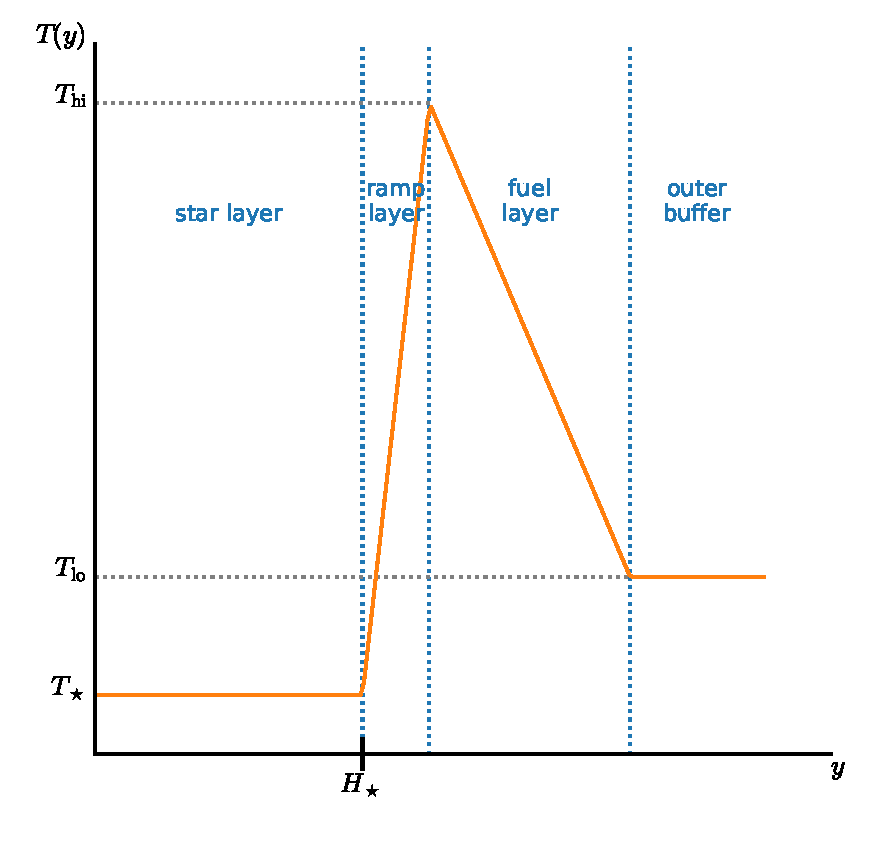
\includegraphics[width=\linewidth]{model}
\caption{\label{fig:sketch} A schematic of our model setup.}
\end{figure}

We wish to create an initial atmosphere consisting of a hot
``post-flame'' region and a cooler atmosphere that the flame will
laterally propagate into.  We put the hot region at the very left of
the domain (the origin of the axisymmetric coordinates).  To create
these initial conditions, w produce two different hydrostatic models,
a ``hot'' model that will represent the perturbation that drives the
flame and a ``cool'' model that will represent the state ahead of the
flame.  These will have different scale heights.  To create these
models, we break the vertical structure of the atmosphere into 4
layers: the underlying star, a ramp-up to the base of the
accreted atmosphere, a fuel layer representing the bulk of the
atmosphere where the flame will propagate, and an outer, low density,
isothermal buffer above the atmosphere that allows us
to capture expansion and explosive dynamics.  This is sketched in
Figure~\ref{fig:sketch}.

The temperature profile in the star and ramp region is given as:
\begin{equation}
T = T_\star + \frac{1}{2} (T_\mathrm{hi} - T_\star) \left [ 1 + \tanh\left( \frac{\tilde{y}}{2 \delta_\mathrm{atm}} \right ) \right ]
\end{equation}
with
\begin{equation}
\tilde{y} = y - H_\star - \frac{3}{2} \delta_\mathrm{atm}
\end{equation}
Here, $\delta_\mathrm{atm}$ is a characteristic width of the transition
ramp, $T_\mathrm{hi}$ is the highest temperature in the HSE model---it
will represent the base of the fuel layer.

The mass fractions use this same profile, switching from a set
describing the underlying star, ${X_k}_\star$, and the set for the
accreted material, ${X_k}_\mathrm{atm}$, which is used in the
isentropic and outer regions.  Note, since the profile above is
linear in $X$, if the initial mass fractions sum to one, then the blended
mass fractions in the ramp region also sum to one.

We specify the density, $\rho_\mathrm{int} = \rho(y = H_\star)$ as the
starting point for the integration of hydrostatic equilibrium.  This
is just below the ramp-up region---this ensures that regardless of
what the peak temperature ($T_\mathrm{hi}$) is, the state beneath the
ramp-up region remains unchanged.  Therefore, we will still be in
lateral equilibrium in the star region.  We will denote the density
where $T = T_\mathrm{hi}$ as $\rho_\mathrm{fuel}$.


Creating the model involves specifying $T_\star$, $T_\mathrm{hi}$,
$T_\mathrm{lo}$, $\rho_\mathrm{int}$, $H_\star$,
$\delta_\mathrm{atm}$, ${X_k}_\star$, and ${X_k}_\mathrm{atm}$.  We
then integrate outwards from the base of the ramp region ($y =
H_\star$), enforcing the discrete form of hydrostatic equilibrium,
Eq.~\ref{eq:hse}.  Integrating upwards, we would find $p_i$ and
$\rho_i$ using a Newton solve together either with the temperature
specified, $T_i = T(p_i, \rho_i, \{X_k\}_i)$ (in the isothermal, ramp,
and buffer layers) or constant entropy, $s_i = s(p_i, \rho_i,
\{X_k\}_i)$, in the fuel layer.  In each case, using the equation of
state.  This follows the procedures described in \citet{ppm-hse}.  We
use the constant temperature for all $y < H_\star +
3\delta_\mathrm{atm}$.  Above this, we switch to isentropic until the
temperature drops to a floor value, $T_\mathrm{lo}$, at which point we
again keep the temperature constant.  The integration of the
atmosphere continues until the density falls to a low density cutoff,
$\rho_\mathrm{cutoff}$.  The material above this height is taken to
have constant density and temperature.

\begin{deluxetable}{lcc}
\tablecaption{\label{table:params} Initial model parameters.}
\tablehead{\colhead{parameter} & \colhead{cool} & \colhead{hot}}
\startdata
$T_\star$       & \multicolumn{2}{c}{$5\times 10^7$~K} \\
$T_\mathrm{hi}$ & $2\times 10^8$~K & $1.2\times 10^9$~K \\
$T_\mathrm{lo}$ & \multicolumn{2}{c}{$10^7$~K} \\
$\rho_\mathrm{int}$ & \multicolumn{2}{c}{$3.43\times 10^6~\gcc$} \\
$\rho_\mathrm{fuel}$\tablenotemark{a} & $2.21\times 10^6~\gcc$ & $1.27\times 10^6~\gcc$ \\
$\rho_\mathrm{cutoff}$ & \multicolumn{2}{c}{$10^{-4}~\gcc$} \\
$g$             & \multicolumn{2}{c}{$-1.5\times 10^{14}~\mathrm{cm~s^{-2}}$} \\
$H_\star$       & \multicolumn{2}{c}{5000~cm} \\
$\delta_\mathrm{atm}$ & \multicolumn{2}{c}{50~cm} \\
$X_\star(\isotm{Fe}{56})\tablenotemark{b}$ & \multicolumn{2}{c}{1.0} \\
$X_\mathrm{atm}(\isotm{He}{4})\tablenotemark{b}$ & \multicolumn{2}{c}{1.0} \\
\enddata
%
\tablenotetext{a}{This is not an input parameter, but instead is
  computed during integration.  We list it here for reference.}
%
\tablenotetext{b}{All other species are taken as 0.}
\end{deluxetable}

The choice of factors in front of $\delta_\mathrm{atm}$ were designed
to make sure the peak $T$ is attained at the desired density 
of the burning layer.

We create two models, a ``cool'' model representing the atmosphere
ahead of the flame and a ``hot'' (or perturbed) model that will
initiate the flame by driving the burning.  The parameters we use for
the model generation are listed in Table~\ref{table:params}.

We blend the hot and cold models laterally to produce the perturbation
needed to initiate a localized flame, with the hot model at the
origin of the axisymmetric geometry.  The blending is done as:
\begin{align}
p(x,y) &= f(x) p_\mathrm{hot}(y) + [1-f(x)] p_\mathrm{cool}(y) \\
\rho(x,y) &= f(x) \rho_\mathrm{hot}(y) + [1-f(x)] \rho_\mathrm{cool}(y) \\
X_k(x,y) &= f(x) {X_k}_\mathrm{hot}(y) + [1-f(x)] {X_k}_\mathrm{cool}(y)
\end{align}
with
\begin{equation}
f(x) = \begin{cases}
     1 & x < x_\mathrm{pert} \\
   1 - \frac{x - x_\mathrm{pert}}{\delta_\mathrm{blend}} & x_\mathrm{pert} \le x \le x_\mathrm{pert} + \delta_\mathrm{blend} \\
     0 & x > x_\mathrm{pert} + \delta_\mathrm{blend}
\end{cases}
\end{equation}
Since the equation of hydrostatic equilibrium is linear and our
blending is a linear combination of two models in hydrostatic
equilibrum, the blended model is also in equilibrium initially.  We choose
$x_\mathrm{pert} = 1.024\times 10^4$~cm and $\delta_\mathrm{blend} = 2048$~cm.  Once
the blended model is constructed, we compute $T(y)$ and $(\rho e)(y)$
from the equation of state.  \MarginPar{show}

\begin{figure}[t]
\centering
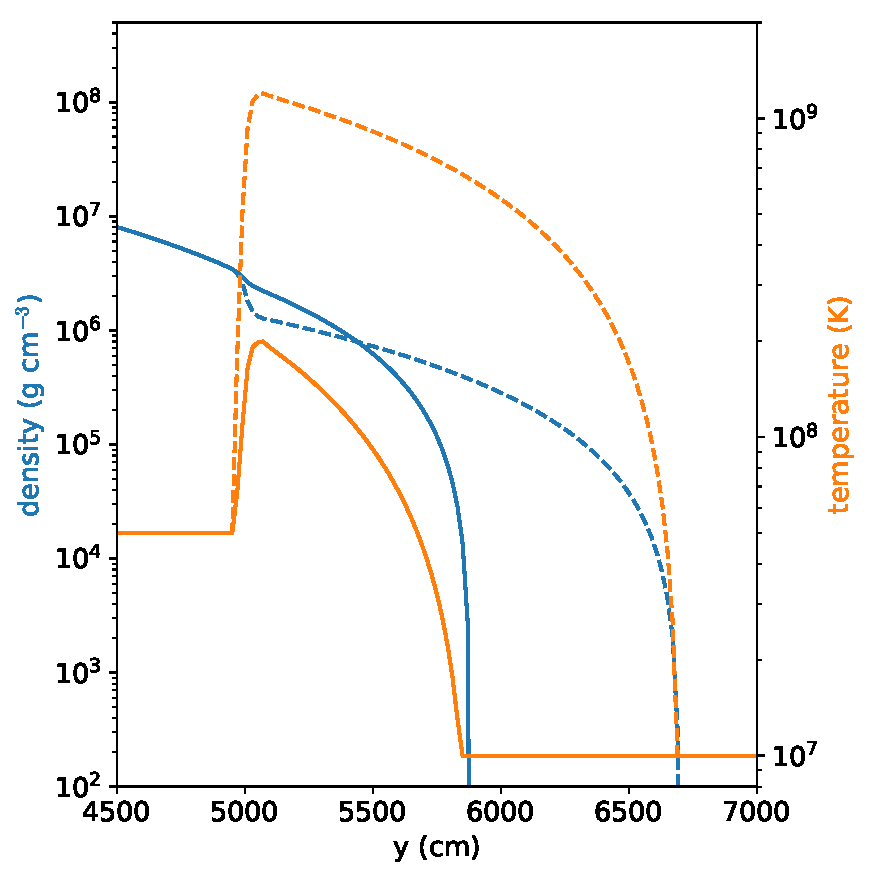
\includegraphics[width=\linewidth]{initial_model_paper}
\caption{\label{fig:initial_models} Our ``cool'' (solid) and ``hot''
  (dashed) initial models, showing both the density and temperature.}
\end{figure}



%======================================================================
% Results
%======================================================================
\section{Simulations and Results}\label{Sec:results}

Things to try to make the model feasible:
\begin{itemize}
\item Start the initial perturbation location near the Rossby radius
\item Hotter ``hot'' model
\item Aprox13
\item Higher diffusion cutoff lessens the timestep restriction
\end{itemize}


All simulations were run with in a domain $8.192\times
10^4~\mathrm{cm} \times 2.048\times 10^4~\mathrm{cm}$.  With our
default refinement, this gives a resolution of $20~\mathrm{cm}$ on the
finest level.  As a comparison, the resolution in our detonation
models was $98~\mathrm{cm}$ and in our multidimensional convection
studies was $6~\mathrm{cm}$.

We specify the rotation period, $P_\mathrm{rot}$, which is related to
the angular rotation rate as $\Omega = 2\pi / P_\mathrm{rot}$.  Our
default rotation period is $0.0005~\mathrm{s}$ (2000 times per
second).  This is quite fast, but picked to make the Rossby length
small enough to fit in the spatial scales we can model.  With this
rotation rate, the Rossby length is
\begin{equation}
L_R = \frac{\sqrt{g H_0}}{\Omega} \sim 3\times 10^4~\mathrm{cm}
\end{equation}
\MarginPar{we should make the width of the hot region closer to the
  Rossby length} using a scale height $H_0 = 10^3~\mathrm{cm}$.  This
is less than half our domain width.

We note that the entire simulation framework for these calculations is 
freely available in the \castro\ github repository.

\subsection{Resolution}

Our default resolution puts $\sim 50$ zones vertically in the ``cool''
model atmosphere height.  To understand the effects of resolution, we
also perform a run with one additional level, with a $2\times$ jump
refining just the region where the density is $10^4~\gcc < \rho \le
4\times 10^4~\gcc$.  On this level, the grid resolution is
$10~\mathrm{cm}$.

\subsection{Rotation Rate}

We also try a rotation period of $P_\mathrm{rot} \sim 10^{-4}~\mathrm{s}$.

\subsection{Reaction Network}

We use aprox13 instead of the small network to understand the
differences.  Energy comes out faster.

\subsection{Boosting}

To meet reasonable timescales, we boosted the microphysical inputs to
the flame to result in a faster flame.  Here we look at the effect of
this choice.

\subsection{Sponge}



\section{Discussion}

Full hydrodynamics models of flame spreading in XRB are possible with certain approximations.

CPU cost

Accurate simulations require
\begin{enumerate}
\item Resolving the scale height of the atmosphere

\item Thin transition between underlying neutron star and atmosphere, to ensure that the peak temperature
hits right at the proper base density
\end{enumerate}

The main approximations we made were
\begin{enumerate}
\item A higher than normal rotation rate
\item A boosted flame
\item Simplified reaction network
\item A 2.5D model for the flow
\end{enumerate}
The first two of these were needed to reduce the spatial and temporal
scales needed to model, making the simulations feasible.  Using the
simulation framework developed here, these both can be relaxed in the
future, at the cost of more computer time.  The same goes for 2.5D
vs.\ full 3D---the only difference is computer time, and our future
calculations will explore the 3D evolution and compare to these.  In particular,
in 3D we will be able to explore shear instabilities at the flame front.
Larger networks are a straightforward change, and already supported in
\castro\ using the \pynucastro\ framework~\citep{pynucastro} and JINA
ReacLib rate database~\citep{reaclib}.

These studies complement the

Other future work includes mixed H/He bursts.  This will require a
different reaction network, and perhaps different (more relaxed)
resolution requirements.

On the algorithmic front, we are exploring a change of our
hydrodynamics and reactive coupling to eliminate splitting error from
the traditional Strang splitting used in \castro\ and other
hydrodynamics codes.  One advantage of this is that the new algorithm
would be more amenable to offloading onto GPUs, a development task
that is underway.  Additionally, we will move to fourth-order accurate
methods and incorporate well-balanced reconstruction to better capture
the burning.

MHD, radiation transport


\acknowledgements \castro\ is open-source and freely available at
\url{http://github.com/AMReX-Astro/Castro}.  The problem setups used
here are available in the git repo as {\tt flame} and {\tt
  flame\_wave}.  The work at Stony Brook was supported by DOE/Office
of Nuclear Physics grant DE-FG02-87ER40317.  This research used
resources of the National Energy Research Scientific Computing Center,
a DOE Office of Science User Facility supported by the Office of
Science of the U.~S.\ Department of Energy under Contract
No.\ DE-AC02-05CH11231.  This research used resources of the Oak Ridge
Leadership Computing Facility at the Oak Ridge National Laboratory,
which is supported by the Office of Science of the U.S. Department of
Energy under Contract No. DE-AC05-00OR22725, awarded through the DOE
INCITE program.

\facilities{NERSC, OLCF}

\software{ADS (http://adsabs.harvard.edu/),
          AMReX (\url{https://github.com/AMReX-Codes/amrex}),
          Castro \citep{castro},
          GCC (\url{https://gcc.gnu.org/}),
          linux (\url{https://www.kernel.org/}),
          matplotlib (\citealt{Hunter:2007}, \url{http://matplotlib.org/}),
          NumPy \citep{numpy,numpy2},
          python (\url{https://www.python.org/}),
          valgrind \citep{valgrind},
          yt \citep{yt}}




\appendix

\section{Diffusion Tests}
\label{app:diffusion}

Show diffusion test problem and convergence.




%======================================================================
% References
%======================================================================

\bibliographystyle{aasjournal}
\bibliography{ws}


\end{document}
